\subsection{Outliers}

The first step in our data evaluation is to check if the data set contains outliers. The different attributes are plotted as box plots, with circles representing the respective outliers.
The used definition of outliers (from the course notes \cite{coursenotes}) is: 

\begin{equation*}
   \text{value} > q_{75} + 1.5 \cdot (q_{75} - q_{25}) \text{ or value} < q_{25} - 1.5 \cdot (q_{75} - q_{25})
\end{equation*}

Even though this definition of outlieres is not definitive, but just a guide, the following visualization is based on the mentioned definition. 

\begin{figure}[H]
    \centering
    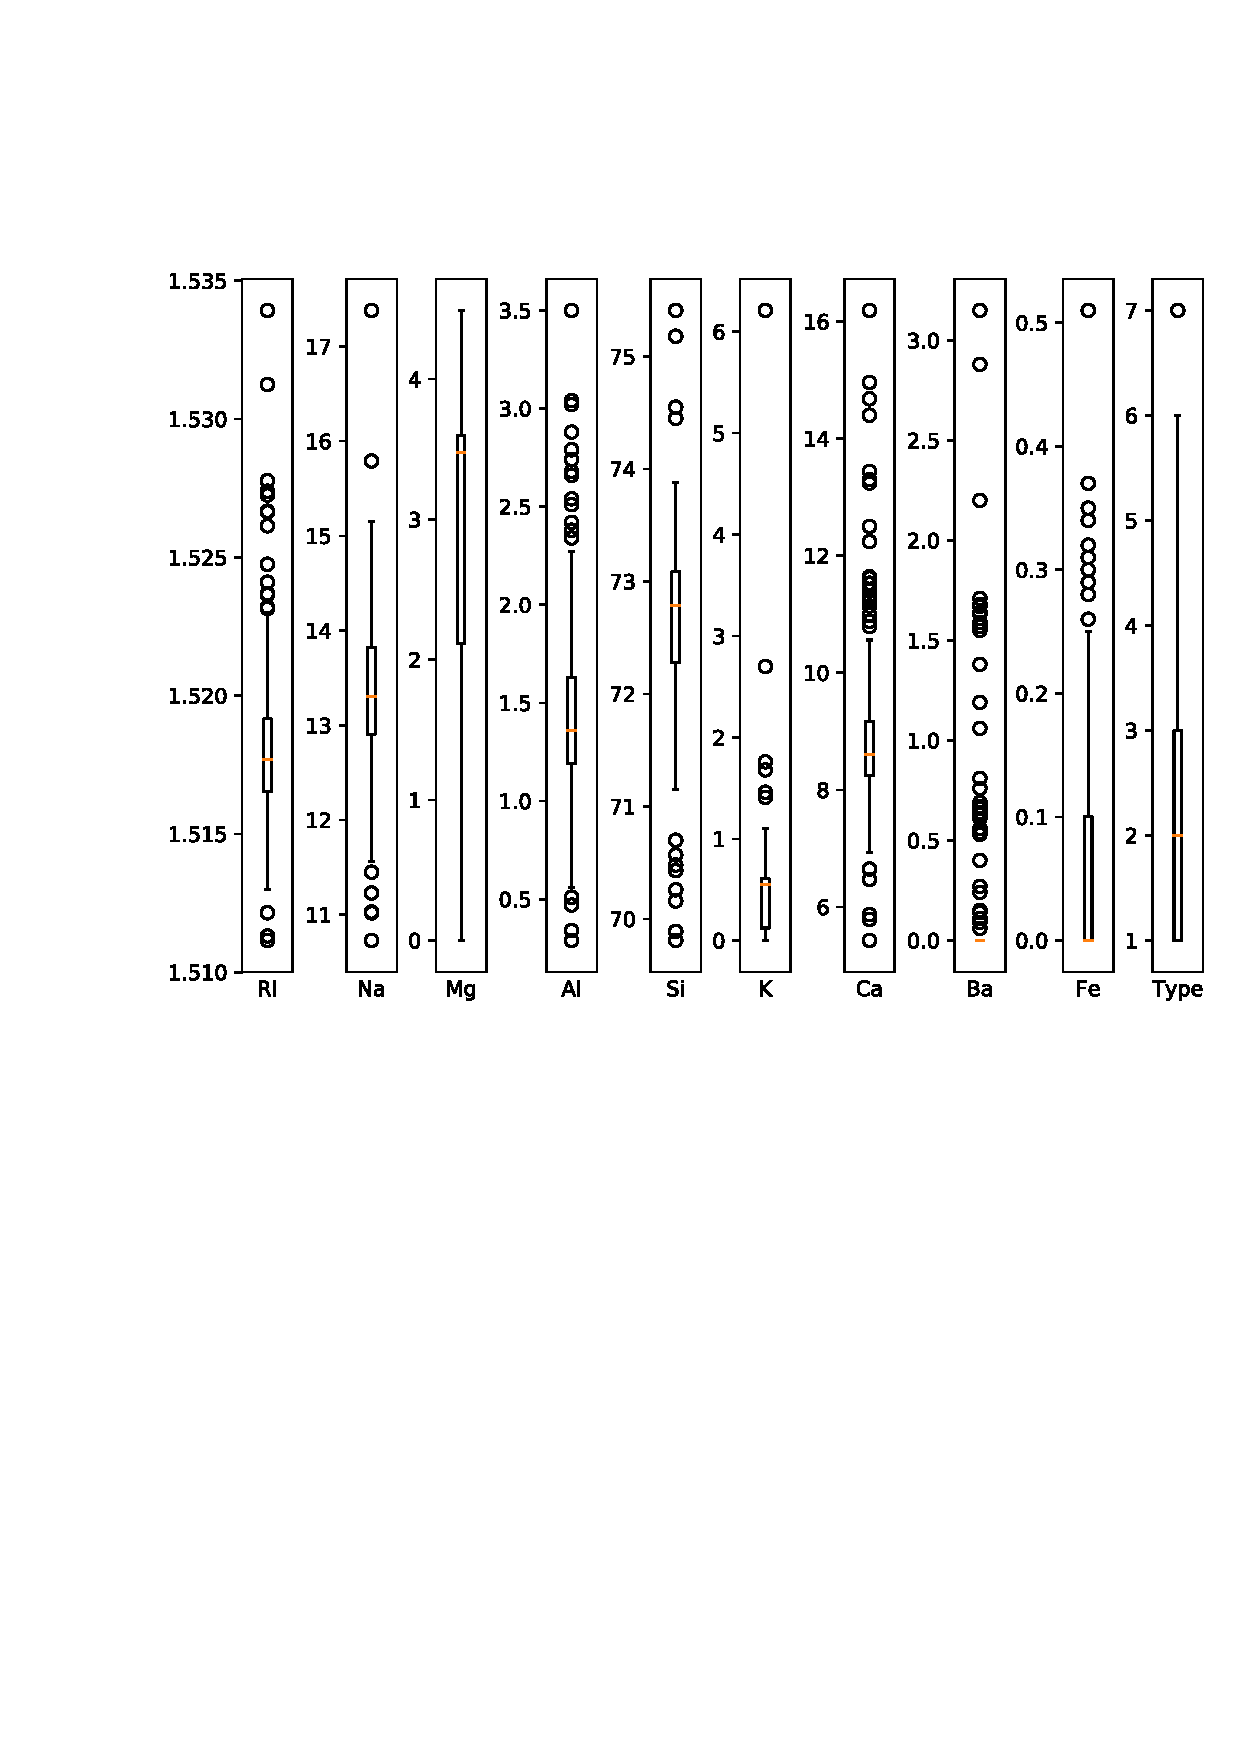
\includegraphics[width=0.8\linewidth]{fig/boxplots.pdf}
    \caption{Box plots with outliers marked by circles.}
    \label{fig:outliers}
\end{figure}

As shown in fig \ref{fig:outliers}, the majority of the attributes contains outliers with respect to the definition mentioned above. The first box plot is the refractive index, the next 8 box plots constitute the contents of the glass, and the final box plot shows the distribution of the different glass types. Since most of the attributes are glass contents, the found outliers might suggest rare compositions of glass, and are therefore valuable for the data set. One box plot which looks peculiar, is the barium (\texttt{Ba}) content, which is majorly dominated by zeros (not present in the observed glass). All cases of barium's presence therefore becomes an outlier.